This section studies how block size and branch prediction limit the performance of core composition.
An analytical model is defined to estimate the performance of a core composition, shown in Equation~\ref{form:wcetMath}.
The variables in Equation~\ref{form:wcetMath} are the average block size \textit{ABS},  the size of the composition \textit{CS} and branch prediction accuracy \textit{BPredAcc} that ranges from 0 to 1.
The constant 2 in Equation~\ref{form:wcetMath} derives from the hardware constraint that a core can execute up to 2 instructions per cycle.
\textit{SyncCost} represents the cost (in cycles) of having to commit blocks sequentially in a core composition, this is covered in more details later on.
This analytical model enables a better understanding of what leads to good performance and how to determine regions of code that benefit from core composition.
The limit study explains why each component of Equation~\ref{form:wcetMath} are important to predict the performance of a core composition.

\begin{align}\label{form:wcetMath}
IPC(ASB,CS,BPredAcc) &= \bigg(\frac{ABS}{SyncCost(ABS,CS) + {\frac{ABS}{2}}}\bigg) \times BPredAcc \times CS
\end{align}


\subsection{Branch Prediction}

As discussed in Chapter~\ref{chp:Background} Section~\ref{chp:Background:sec:EDGE}, an EDGE based DMP accelerates a single thread by executing blocks of instructions from the same thread speculatively across several fused cores. 
In a core composition, the fetching scheme dictates that a core must fetch blocks until its instruction window is either full or cannot accomodate the newest block.
Once this requirement is met, the following block is sent to the next core in the composition.
If a core mispeculates a block, this can cause the entire composition to be flushed.
Thus core composition puts a strain on the branch predictor since efficiently using the cores depends on the prediction accuracy.

Depending on the sizes of the blocks and the number of cores in the composition, the branch predictor has to meet a different accuracy requirement in order to ensure that all cores are being used efficiently.
In this case, efficiency is defined by cores in a composition fetching blocks from the correct branch path, meaning cores in the composition are executing useful code.
Given a core-composition of size \textit{CompSize} and average block size \textit{ABS}, the minimum branch prediction accuracy required to ensure efficient use of the composition can be determined using Formula~\ref{form:minpred} where \textit{BlocksInFlight} can be calculated using the equation~\ref{form:blocks}.
The groups in the Equation are derived from hardware limitations: the instruction window is divided into 4 lanes that can take a block of up to 32 instructions each.

\begin{equation}\label{form:blocks}
BlocksInFlight(AverageBlockSize) = \begin{cases}
4, &\text{if } AverageBlockSize \le 32 \\
3, &\text{if } 32 < AverageBlockSize \le 64 \\
2, &\text{if } 64 < AverageBlockSize \le 96\\
1, &\text{if } 96 < AverageBlockSize\\
\end{cases}
\end{equation}

\begin{equation}\label{form:minpred}
RequiredAccuracy(ABS,CompSize)= \frac{BlocksInFlight(ABS) \times CompSize- 1}{BlocksInFlight(ABS) \times CompSize}
\vspace{1em}
\end{equation}


Given an average size of a block being executed in a program (\textit{ABS}) and a core composition of size (\textit{CompSize}), the branch prediction accuracy required to ensure that each core in the composition is executing a block on the correct branch path can be calculated using Equation~\ref{form:minpred}.
In Equation~\ref{form:minpred}, the -1 is due to the fact that when a program is executing the first block does not depend on a branch prediction, thus at any point during the execution of a program, there is a non-speculative block that does not need to predicted.

\begin{figure}[t]
    \centering
    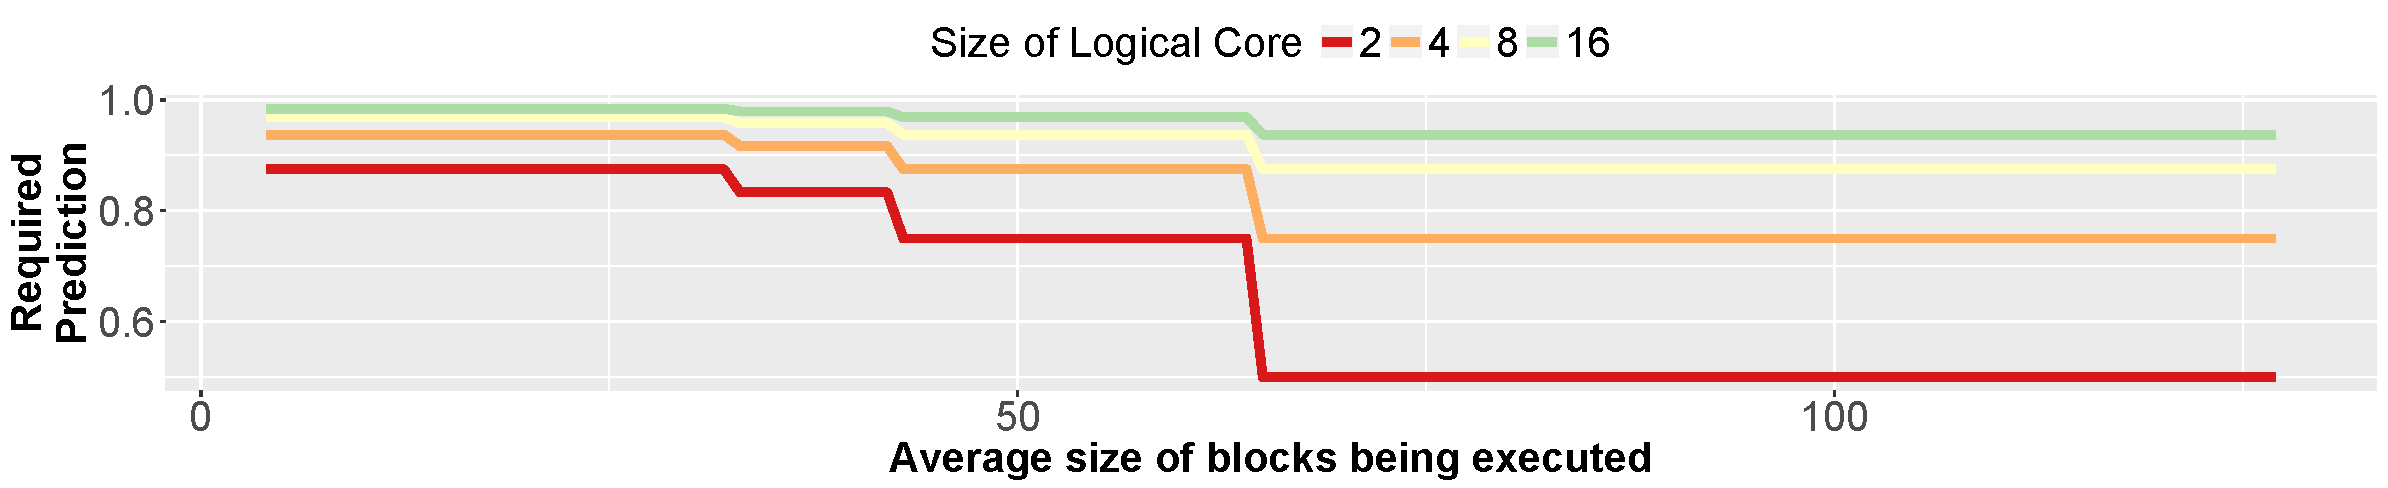
\includegraphics[width=\textwidth]{cases-paper/graphics/limit_study/prediction_req.pdf}
    \caption{Required prediction accuracy for a logical core size to be efficient given an average block size.}
    \label{fig:req_pred}
	\vspace{1em}
\end{figure}
Figure~\ref{fig:req_pred} plots the results of using Equation~\ref{form:minpred} with different block sizes and core composition sizes.
Adding extra physical cores to a composition requires an increasingly accurate branch predictor, especially when the size of a block is under 50 instructions.
This provides two insights; first of all large LCs will need to run on code sections with less control flow as they are more sensitive to branch misspredictions.
Second of all, branch prediction can be a simple method of evaluating the current effectiveness of a core composition.
Given a certain number of cores, if the prediction accuracy is under the limits presented in Figure~\ref{fig:req_pred} it can be easily determine that the core composition size is sub-optimal.

\subsection{Synchronization Cost}

For a program to execute correctly, the cores in a composition must communicate when they have finished executing a block.
This ensures that the cores fetch blocks from the correct control paths and update memory and registers consistently.
A core may have to wait for other cores to commit before fetching a new block. 
The worst-case estimate of this stall is defined as the \textbf{Synchronization Cost}.

\begin{equation}\label{form:synccost}
SyncCos(ABS,CompSize) = \frac{\sum_{CoreID=0}^{CompSize-1}\left(BlocksInFlight(ABS)\right) \times CoreID }{CompSize}
\end{equation}


Blocks commit in a sequential fashion with the non-speculative block committing first and the most recent speculative block committing last.
If a core's instruction window is full then it must commit a block before it fetches a new one.
The Synchronization Cost, in cycles, is defined in equation~\ref{form:synccost} and is measured by averaging the overall number of cycles each fused core waits until it can continue to fetch and execute new blocks.
\textit{AvBlocksInFlight} represents the average number of blocks in flight on a single core in the composition.
This is a worst-case estimate as block sizes will fluctuate during the execution of a program.

Figure~\ref{fig:sync_cost} shows how many cycles the Synchronization Cost will be for a given core composition size and average block size.
The larger the block size the lower the Synchronization Cost is since cores fetch fewer blocks and wait less for other fused cores to finish committing.
Large LCs executing small blocks have a high Synchronization Cost. 
This indicates that large LCs should be avoided when dealing with smaller blocks as the Synchronization Cost outweighs the code execution.

\begin{figure}[t]
    \centering
    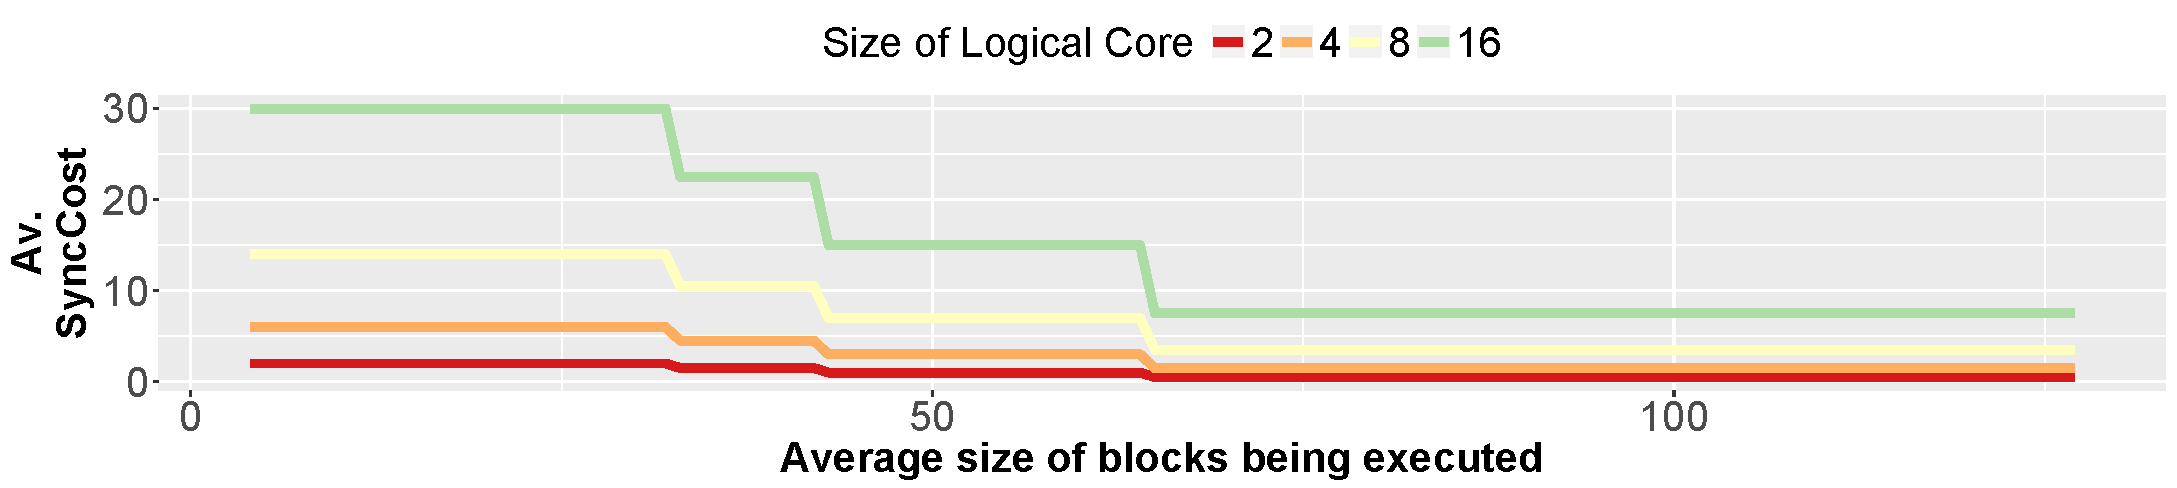
\includegraphics[width=\textwidth]{cases-paper/graphics/limit_study/sync_cost.pdf}

    \caption{Synchronization Cost in cycles for a given number of cores in a composition and an average block size.} %Each core has 4 lanes and each lane can fetch a block of up to 32 instructions. Lower is better.}
    \label{fig:sync_cost}
	\vspace{1em}
\end{figure}


\begin{figure}[t]
    \centering
    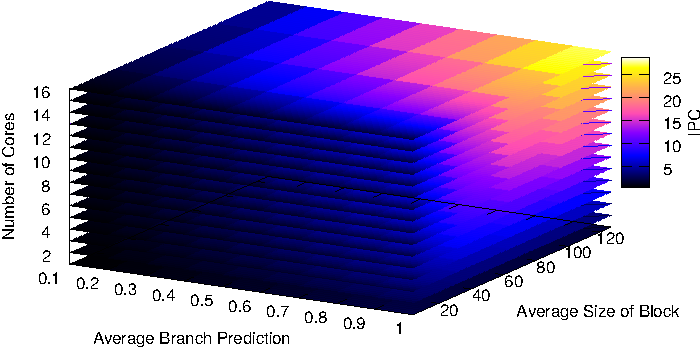
\includegraphics[width=0.8\textwidth]{cases-paper/graphics/limit_study/summary.pdf}
    \caption{IPC estimate given a logical processor size, average branch prediction and average block size for a dual-issue core. A higher IPC means better performance.}
    \label{fig:lm_summ}
\vspace{5mm}
\end{figure}

\paragraph{Summary}

This section estimates the worst-case IPC for a logical processor using Average Block Size, Average Branch Prediction, and Synchonization Cost using the analytical model presented in Equation~\ref{form:wcetMath}.
Figure~\ref{fig:lm_summ} presented a worst-case estimate of IPC performance assuming each core can sustain an IPC of 2.
The figure is generated by assuming that cores can execute 2 instructions per block, and using Equation~\ref{form:wcetMath} with different block sizes, accuracies and core composition sizes to generate estimated IPC values.
From what was previously explained, Figure~\ref{fig:lm_summ} shows that to obtain optimal performance requires a high branch prediction accuracy and large blocks.
It shows that larger logical processors can easily under-perform; for example it can be seen that 16 fused cores often have IPCs under 15, meaning that each core has an IPC under~1.

